\documentclass[11pt]{article}
\newcommand{\tablelang}{en}
% Shared preamble for docs/paper/tex/en/main.tex and docs/paper/tex/uk/main.tex (XeLaTeX via Tectonic).
% Same layout, fonts and packages as the author's earlier Zenodo preprint (10.5281/zenodo.23375871).
% The including file sets \mainlang{english} or \mainlang{ukrainian} before % Shared preamble for docs/paper/tex/en/main.tex and docs/paper/tex/uk/main.tex (XeLaTeX via Tectonic).
% Same layout, fonts and packages as the author's earlier Zenodo preprint (10.5281/zenodo.23375871).
% The including file sets \mainlang{english} or \mainlang{ukrainian} before % Shared preamble for docs/paper/tex/en/main.tex and docs/paper/tex/uk/main.tex (XeLaTeX via Tectonic).
% Same layout, fonts and packages as the author's earlier Zenodo preprint (10.5281/zenodo.23375871).
% The including file sets \mainlang{english} or \mainlang{ukrainian} before \input{../preamble}.
\usepackage[a4paper,margin=25mm]{geometry}
\usepackage{fontspec}
\setmainfont{cmunrm.otf}[BoldFont=cmunbx.otf,ItalicFont=cmunti.otf,BoldItalicFont=cmunbi.otf]
\setsansfont{cmunss.otf}[BoldFont=cmunsx.otf,ItalicFont=cmunsi.otf]
\setmonofont{cmuntt.otf}[BoldFont=cmuntb.otf,ItalicFont=cmunit.otf]
\usepackage[ukrainian,english]{babel}
\usepackage{amsmath,amssymb,amsthm,mathtools}
\usepackage{booktabs,tabularx,array,multirow}
\usepackage{graphicx}
\usepackage[font=small,labelfont=bf]{caption}
\usepackage{subcaption}
\usepackage{xcolor}
\usepackage{microtype}
\usepackage[numbers,sort&compress]{natbib}
\PassOptionsToPackage{hyphens}{url}
\usepackage[hidelinks]{hyperref}
\usepackage[nameinlink,capitalise,noabbrev]{cleveref}
\usepackage{url}
\usepackage{etoolbox}
\AtBeginEnvironment{thebibliography}{\raggedright}

\graphicspath{{../../figures/}}
% primitive input: LaTeX's \input is not expandable and breaks inside tabular after \midrule
\makeatletter\newcommand{\gentable}[1]{\@@input ../tables/\tablelang/T#1.tex }\makeatother

% theorem names: the including file may define these before \input{../preamble}
\providecommand{\lemmaname}{Lemma}
\providecommand{\propositionname}{Proposition}
\providecommand{\definitionname}{Definition}
\providecommand{\remarkname}{Remark}
\providecommand{\corollaryname}{Corollary}
\providecommand{\theoremname}{Theorem}
\theoremstyle{plain}
\newtheorem{lemma}{\lemmaname}
\newtheorem{proposition}{\propositionname}
\theoremstyle{definition}
\newtheorem{definition}{\definitionname}
\theoremstyle{remark}
\newtheorem{remark}{\remarkname}

\setlength{\tabcolsep}{4pt}
\renewcommand{\arraystretch}{1.12}
\newcommand{\code}[1]{\texttt{#1}}
\sloppy
.
\usepackage[a4paper,margin=25mm]{geometry}
\usepackage{fontspec}
\setmainfont{cmunrm.otf}[BoldFont=cmunbx.otf,ItalicFont=cmunti.otf,BoldItalicFont=cmunbi.otf]
\setsansfont{cmunss.otf}[BoldFont=cmunsx.otf,ItalicFont=cmunsi.otf]
\setmonofont{cmuntt.otf}[BoldFont=cmuntb.otf,ItalicFont=cmunit.otf]
\usepackage[ukrainian,english]{babel}
\usepackage{amsmath,amssymb,amsthm,mathtools}
\usepackage{booktabs,tabularx,array,multirow}
\usepackage{graphicx}
\usepackage[font=small,labelfont=bf]{caption}
\usepackage{subcaption}
\usepackage{xcolor}
\usepackage{microtype}
\usepackage[numbers,sort&compress]{natbib}
\PassOptionsToPackage{hyphens}{url}
\usepackage[hidelinks]{hyperref}
\usepackage[nameinlink,capitalise,noabbrev]{cleveref}
\usepackage{url}
\usepackage{etoolbox}
\AtBeginEnvironment{thebibliography}{\raggedright}

\graphicspath{{../../figures/}}
% primitive input: LaTeX's \input is not expandable and breaks inside tabular after \midrule
\makeatletter\newcommand{\gentable}[1]{\@@input ../tables/\tablelang/T#1.tex }\makeatother

% theorem names: the including file may define these before % Shared preamble for docs/paper/tex/en/main.tex and docs/paper/tex/uk/main.tex (XeLaTeX via Tectonic).
% Same layout, fonts and packages as the author's earlier Zenodo preprint (10.5281/zenodo.23375871).
% The including file sets \mainlang{english} or \mainlang{ukrainian} before \input{../preamble}.
\usepackage[a4paper,margin=25mm]{geometry}
\usepackage{fontspec}
\setmainfont{cmunrm.otf}[BoldFont=cmunbx.otf,ItalicFont=cmunti.otf,BoldItalicFont=cmunbi.otf]
\setsansfont{cmunss.otf}[BoldFont=cmunsx.otf,ItalicFont=cmunsi.otf]
\setmonofont{cmuntt.otf}[BoldFont=cmuntb.otf,ItalicFont=cmunit.otf]
\usepackage[ukrainian,english]{babel}
\usepackage{amsmath,amssymb,amsthm,mathtools}
\usepackage{booktabs,tabularx,array,multirow}
\usepackage{graphicx}
\usepackage[font=small,labelfont=bf]{caption}
\usepackage{subcaption}
\usepackage{xcolor}
\usepackage{microtype}
\usepackage[numbers,sort&compress]{natbib}
\PassOptionsToPackage{hyphens}{url}
\usepackage[hidelinks]{hyperref}
\usepackage[nameinlink,capitalise,noabbrev]{cleveref}
\usepackage{url}
\usepackage{etoolbox}
\AtBeginEnvironment{thebibliography}{\raggedright}

\graphicspath{{../../figures/}}
% primitive input: LaTeX's \input is not expandable and breaks inside tabular after \midrule
\makeatletter\newcommand{\gentable}[1]{\@@input ../tables/\tablelang/T#1.tex }\makeatother

% theorem names: the including file may define these before \input{../preamble}
\providecommand{\lemmaname}{Lemma}
\providecommand{\propositionname}{Proposition}
\providecommand{\definitionname}{Definition}
\providecommand{\remarkname}{Remark}
\providecommand{\corollaryname}{Corollary}
\providecommand{\theoremname}{Theorem}
\theoremstyle{plain}
\newtheorem{lemma}{\lemmaname}
\newtheorem{proposition}{\propositionname}
\theoremstyle{definition}
\newtheorem{definition}{\definitionname}
\theoremstyle{remark}
\newtheorem{remark}{\remarkname}

\setlength{\tabcolsep}{4pt}
\renewcommand{\arraystretch}{1.12}
\newcommand{\code}[1]{\texttt{#1}}
\sloppy

\providecommand{\lemmaname}{Lemma}
\providecommand{\propositionname}{Proposition}
\providecommand{\definitionname}{Definition}
\providecommand{\remarkname}{Remark}
\providecommand{\corollaryname}{Corollary}
\providecommand{\theoremname}{Theorem}
\theoremstyle{plain}
\newtheorem{lemma}{\lemmaname}
\newtheorem{proposition}{\propositionname}
\theoremstyle{definition}
\newtheorem{definition}{\definitionname}
\theoremstyle{remark}
\newtheorem{remark}{\remarkname}

\setlength{\tabcolsep}{4pt}
\renewcommand{\arraystretch}{1.12}
\newcommand{\code}[1]{\texttt{#1}}
\sloppy
.
\usepackage[a4paper,margin=25mm]{geometry}
\usepackage{fontspec}
\setmainfont{cmunrm.otf}[BoldFont=cmunbx.otf,ItalicFont=cmunti.otf,BoldItalicFont=cmunbi.otf]
\setsansfont{cmunss.otf}[BoldFont=cmunsx.otf,ItalicFont=cmunsi.otf]
\setmonofont{cmuntt.otf}[BoldFont=cmuntb.otf,ItalicFont=cmunit.otf]
\usepackage[ukrainian,english]{babel}
\usepackage{amsmath,amssymb,amsthm,mathtools}
\usepackage{booktabs,tabularx,array,multirow}
\usepackage{graphicx}
\usepackage[font=small,labelfont=bf]{caption}
\usepackage{subcaption}
\usepackage{xcolor}
\usepackage{microtype}
\usepackage[numbers,sort&compress]{natbib}
\PassOptionsToPackage{hyphens}{url}
\usepackage[hidelinks]{hyperref}
\usepackage[nameinlink,capitalise,noabbrev]{cleveref}
\usepackage{url}
\usepackage{etoolbox}
\AtBeginEnvironment{thebibliography}{\raggedright}

\graphicspath{{../../figures/}}
% primitive input: LaTeX's \input is not expandable and breaks inside tabular after \midrule
\makeatletter\newcommand{\gentable}[1]{\@@input ../tables/\tablelang/T#1.tex }\makeatother

% theorem names: the including file may define these before % Shared preamble for docs/paper/tex/en/main.tex and docs/paper/tex/uk/main.tex (XeLaTeX via Tectonic).
% Same layout, fonts and packages as the author's earlier Zenodo preprint (10.5281/zenodo.23375871).
% The including file sets \mainlang{english} or \mainlang{ukrainian} before % Shared preamble for docs/paper/tex/en/main.tex and docs/paper/tex/uk/main.tex (XeLaTeX via Tectonic).
% Same layout, fonts and packages as the author's earlier Zenodo preprint (10.5281/zenodo.23375871).
% The including file sets \mainlang{english} or \mainlang{ukrainian} before \input{../preamble}.
\usepackage[a4paper,margin=25mm]{geometry}
\usepackage{fontspec}
\setmainfont{cmunrm.otf}[BoldFont=cmunbx.otf,ItalicFont=cmunti.otf,BoldItalicFont=cmunbi.otf]
\setsansfont{cmunss.otf}[BoldFont=cmunsx.otf,ItalicFont=cmunsi.otf]
\setmonofont{cmuntt.otf}[BoldFont=cmuntb.otf,ItalicFont=cmunit.otf]
\usepackage[ukrainian,english]{babel}
\usepackage{amsmath,amssymb,amsthm,mathtools}
\usepackage{booktabs,tabularx,array,multirow}
\usepackage{graphicx}
\usepackage[font=small,labelfont=bf]{caption}
\usepackage{subcaption}
\usepackage{xcolor}
\usepackage{microtype}
\usepackage[numbers,sort&compress]{natbib}
\PassOptionsToPackage{hyphens}{url}
\usepackage[hidelinks]{hyperref}
\usepackage[nameinlink,capitalise,noabbrev]{cleveref}
\usepackage{url}
\usepackage{etoolbox}
\AtBeginEnvironment{thebibliography}{\raggedright}

\graphicspath{{../../figures/}}
% primitive input: LaTeX's \input is not expandable and breaks inside tabular after \midrule
\makeatletter\newcommand{\gentable}[1]{\@@input ../tables/\tablelang/T#1.tex }\makeatother

% theorem names: the including file may define these before \input{../preamble}
\providecommand{\lemmaname}{Lemma}
\providecommand{\propositionname}{Proposition}
\providecommand{\definitionname}{Definition}
\providecommand{\remarkname}{Remark}
\providecommand{\corollaryname}{Corollary}
\providecommand{\theoremname}{Theorem}
\theoremstyle{plain}
\newtheorem{lemma}{\lemmaname}
\newtheorem{proposition}{\propositionname}
\theoremstyle{definition}
\newtheorem{definition}{\definitionname}
\theoremstyle{remark}
\newtheorem{remark}{\remarkname}

\setlength{\tabcolsep}{4pt}
\renewcommand{\arraystretch}{1.12}
\newcommand{\code}[1]{\texttt{#1}}
\sloppy
.
\usepackage[a4paper,margin=25mm]{geometry}
\usepackage{fontspec}
\setmainfont{cmunrm.otf}[BoldFont=cmunbx.otf,ItalicFont=cmunti.otf,BoldItalicFont=cmunbi.otf]
\setsansfont{cmunss.otf}[BoldFont=cmunsx.otf,ItalicFont=cmunsi.otf]
\setmonofont{cmuntt.otf}[BoldFont=cmuntb.otf,ItalicFont=cmunit.otf]
\usepackage[ukrainian,english]{babel}
\usepackage{amsmath,amssymb,amsthm,mathtools}
\usepackage{booktabs,tabularx,array,multirow}
\usepackage{graphicx}
\usepackage[font=small,labelfont=bf]{caption}
\usepackage{subcaption}
\usepackage{xcolor}
\usepackage{microtype}
\usepackage[numbers,sort&compress]{natbib}
\PassOptionsToPackage{hyphens}{url}
\usepackage[hidelinks]{hyperref}
\usepackage[nameinlink,capitalise,noabbrev]{cleveref}
\usepackage{url}
\usepackage{etoolbox}
\AtBeginEnvironment{thebibliography}{\raggedright}

\graphicspath{{../../figures/}}
% primitive input: LaTeX's \input is not expandable and breaks inside tabular after \midrule
\makeatletter\newcommand{\gentable}[1]{\@@input ../tables/\tablelang/T#1.tex }\makeatother

% theorem names: the including file may define these before % Shared preamble for docs/paper/tex/en/main.tex and docs/paper/tex/uk/main.tex (XeLaTeX via Tectonic).
% Same layout, fonts and packages as the author's earlier Zenodo preprint (10.5281/zenodo.23375871).
% The including file sets \mainlang{english} or \mainlang{ukrainian} before \input{../preamble}.
\usepackage[a4paper,margin=25mm]{geometry}
\usepackage{fontspec}
\setmainfont{cmunrm.otf}[BoldFont=cmunbx.otf,ItalicFont=cmunti.otf,BoldItalicFont=cmunbi.otf]
\setsansfont{cmunss.otf}[BoldFont=cmunsx.otf,ItalicFont=cmunsi.otf]
\setmonofont{cmuntt.otf}[BoldFont=cmuntb.otf,ItalicFont=cmunit.otf]
\usepackage[ukrainian,english]{babel}
\usepackage{amsmath,amssymb,amsthm,mathtools}
\usepackage{booktabs,tabularx,array,multirow}
\usepackage{graphicx}
\usepackage[font=small,labelfont=bf]{caption}
\usepackage{subcaption}
\usepackage{xcolor}
\usepackage{microtype}
\usepackage[numbers,sort&compress]{natbib}
\PassOptionsToPackage{hyphens}{url}
\usepackage[hidelinks]{hyperref}
\usepackage[nameinlink,capitalise,noabbrev]{cleveref}
\usepackage{url}
\usepackage{etoolbox}
\AtBeginEnvironment{thebibliography}{\raggedright}

\graphicspath{{../../figures/}}
% primitive input: LaTeX's \input is not expandable and breaks inside tabular after \midrule
\makeatletter\newcommand{\gentable}[1]{\@@input ../tables/\tablelang/T#1.tex }\makeatother

% theorem names: the including file may define these before \input{../preamble}
\providecommand{\lemmaname}{Lemma}
\providecommand{\propositionname}{Proposition}
\providecommand{\definitionname}{Definition}
\providecommand{\remarkname}{Remark}
\providecommand{\corollaryname}{Corollary}
\providecommand{\theoremname}{Theorem}
\theoremstyle{plain}
\newtheorem{lemma}{\lemmaname}
\newtheorem{proposition}{\propositionname}
\theoremstyle{definition}
\newtheorem{definition}{\definitionname}
\theoremstyle{remark}
\newtheorem{remark}{\remarkname}

\setlength{\tabcolsep}{4pt}
\renewcommand{\arraystretch}{1.12}
\newcommand{\code}[1]{\texttt{#1}}
\sloppy

\providecommand{\lemmaname}{Lemma}
\providecommand{\propositionname}{Proposition}
\providecommand{\definitionname}{Definition}
\providecommand{\remarkname}{Remark}
\providecommand{\corollaryname}{Corollary}
\providecommand{\theoremname}{Theorem}
\theoremstyle{plain}
\newtheorem{lemma}{\lemmaname}
\newtheorem{proposition}{\propositionname}
\theoremstyle{definition}
\newtheorem{definition}{\definitionname}
\theoremstyle{remark}
\newtheorem{remark}{\remarkname}

\setlength{\tabcolsep}{4pt}
\renewcommand{\arraystretch}{1.12}
\newcommand{\code}[1]{\texttt{#1}}
\sloppy

\providecommand{\lemmaname}{Lemma}
\providecommand{\propositionname}{Proposition}
\providecommand{\definitionname}{Definition}
\providecommand{\remarkname}{Remark}
\providecommand{\corollaryname}{Corollary}
\providecommand{\theoremname}{Theorem}
\theoremstyle{plain}
\newtheorem{lemma}{\lemmaname}
\newtheorem{proposition}{\propositionname}
\theoremstyle{definition}
\newtheorem{definition}{\definitionname}
\theoremstyle{remark}
\newtheorem{remark}{\remarkname}

\setlength{\tabcolsep}{4pt}
\renewcommand{\arraystretch}{1.12}
\newcommand{\code}[1]{\texttt{#1}}
\sloppy


% ---- additions local to the English article (preamble.tex left unchanged) ----
\newcolumntype{L}{>{\raggedright\arraybackslash}X}
\newcolumntype{R}{>{\raggedleft\arraybackslash}X}
\newcolumntype{P}[1]{>{\raggedright\arraybackslash}p{#1}}
\crefname{appendix}{Appendix}{Appendices}
\setlength{\emergencystretch}{2em}
\hypersetup{pdftitle={Beyond Passing Tests: An Interface-Only Specification Review Cuts Silent Failures of a Local Gemma Coding Agent},
  pdfauthor={Oleksandr Pylypenko},
  pdfkeywords={coding agents, large language models, specification-based testing, silent failures, Gemma, Gemini, Google Antigravity, pre-registration}}

\begin{document}
\selectlanguage{english}

\title{Beyond Passing Tests: An Interface-Only Specification Review Cuts Silent Failures of a Local Gemma Coding Agent}
\author{Oleksandr Pylypenko\\[2pt]\small Independent Researcher in Artificial Intelligence and Machine Learning\\ \small PhD Student, State University of Trade and Economics, Kyiv, Ukraine\\ \small In cooperation with the Department of Software Engineering and Cybersecurity\\[2pt]
\small ORCID: \href{https://orcid.org/0009-0004-9610-9242}{0009-0004-9610-9242}\\ \small\href{mailto:O.Pylypenko@knute.edu.ua}{\texttt{O.Pylypenko@knute.edu.ua}}}
\date{2026-10-21}
\maketitle

\begin{abstract}
\noindent
Coding agents usually stop when available tests pass, even when those tests omit stated requirements. We study this failure in a cloud-architect/local-builder arrangement with \code{gemma4:12b} repairing small Python modules on a consumer laptop GPU. A cloud reviewer receives only signatures, docstrings and data-type fields, never function bodies, and returns contract tests or a checklist. A separate hidden evaluation scores the resulting code. Across 50 task instances and 150 paired runs with corrected measurement, the contract-test arm reduced silent false successes from 37 to 4 and raised verified completion from 66.0\% to 87.3\%; task-level silent failures fell on 12 instances and rose on none ($p=0.0005$, post hoc). These are pooled, partly development-reused tasks, not 50 independent new specifications. In a pre-registered campaign on 25 new tasks, both review forms raised verified completion from 58/75 to 71/75 and reduced silent false successes from 9/75 to 1/75. The checklist matched the aggregate verified-completion rate of contract tests; equivalence was not tested. Including one generation per task reused across three seeds, campaign time increased by 11.8\% for the checklist and 53.7\% for tests. The registered task-level test did not reach significance ($p=0.125$); the contract-test gains were concentrated in multi-file tasks. An exploratory disclosure ablation points to the importance of docstrings. The results support specification review in this bounded setting, while leaving its causal components and performance on real repository defects unresolved.
\end{abstract}

\noindent\textbf{Keywords:} coding agents; large language models; specification-based testing; test oracles; silent failures; Gemma; Gemini; Google Antigravity; pre-registration.

\medskip
\noindent\textbf{Independence statement.} This study evaluates an architecture pattern that Google has described publicly; it was not coordinated with, sponsored by, or reviewed by Google, and no claim is made about Google's own products beyond the cited announcement. All experiments ran on the author's hardware and accounts.

% =====================================================================
\section{Introduction}\label{sec:intro}
A passing test suite is the usual stopping criterion for an autonomous coding agent. It is also a weak one: when tests cover only part of the specification, an agent can satisfy the tests while violating the rest. Benchmark studies have shown that insufficient tests overstate the correctness of generated code; extending HumanEval's tests reduced pass@$k$ by up to 19.3--28.9\% across 26 models~\citep{liu2023evalplus}. For an agent that works unattended, the failure is worse than a visible error: the agent reports success, and nothing downstream objects.

We met this failure while building a hybrid orchestrator in which a cloud ``architect'' plans and a local model does the editing, so that source code stays on the machine. This is the arrangement Google introduced for local models in the Antigravity SDK: a cloud Gemini model plans from file names and descriptions alone, while local Gemma instances do the work on the device~\citep{kotwani2026antigravity}. With a 12B local worker, the dominant failure on specification-heavy repair tasks was not inability to edit code or to follow a plan: the worker made the visible tests pass and silently missed rules stated only in the docstring. Generation-limit escalation, thinking on retry, cloud guidance after a failed attempt and one-step harness adaptation did not change that (\cref{sec:res-negative}).

This paper asks a narrow question: \textbf{can a cloud model that reads only the specification --- writing contract tests or a checklist of rules --- reduce silent failures of a local coding agent, without the implementation leaving the machine, and at what cost?} Our contributions are:
\begin{enumerate}
\item A measurement of silent false successes of a local coding agent on specification-heavy repair tasks, with an independent hidden evaluation as ground truth.
\item A privacy-bounded mechanism in which the cloud sees signatures, docstrings and data-type fields only, with evidence that interface completeness decides whether contract tests help or harm.
\item A pre-registered campaign with a checklist control that tests whether making the review executable adds measurable benefit, and a construction procedure (seeded rule visibility; bugs written by the local model) that reduces author discretion over where the method can help.
\item An evaluation that separates run-level from task-level inference, reports negative results for five alternative interventions, and checks the generated tests for over-constraint and mutation coverage without involving the agent.
\end{enumerate}
We do not claim that generating tests with language models is new (\cref{sec:related}), nor that the effect generalises beyond the task family studied here (\cref{sec:limitations}).

% =====================================================================
\section{Related work}\label{sec:related}
\paragraph{Insufficient tests.} EvalPlus extended HumanEval's test inputs about 80-fold with LLM- and mutation-based generation and found many solutions previously counted as correct to be wrong~\citep{liu2023evalplus}. Our hidden evaluations play the role of the stronger tests; our concern is the agent's own stopping criterion rather than benchmark scoring.

\paragraph{Tests generated by language models.} CodeT generates tests with the same model that writes candidate solutions and ranks the solutions by agreement with those tests~\citep{chen2023codet}. AgentCoder separates a programmer agent from a test-designer agent that writes tests from the requirements~\citep{huang2024agentcoder}. TestGen-LLM at Meta improves existing human-written test classes and keeps only candidates that pass filters for measurable improvement; in deployment 75\% of its test cases built correctly, 57\% passed reliably and 25\% increased coverage~\citep{alshahwan2024testgen}. Closest to our setting, spec-driven test generation at Google first derives pre-conditions, post-conditions and undefined behaviour and then writes tests from them, improving bug detection on production bugs by 9.8 percentage points ($p=0.0352$)~\citep{tufano2026contracts}. Our mechanism differs in where information flows: the test writer is a \emph{different, remote} model that never sees function bodies, and the tests act as an acceptance gate for a \emph{local} agent rather than as a test-suite product.

\paragraph{Agents that game tests.} ImpossibleBench modifies tests so that they contradict the natural-language specification and measures how often agents nevertheless make them pass~\citep{zhong2026impossiblebench}. Our failure mode is complementary: the agent does not manipulate tests; it stops when the visible tests pass and leaves rules that the tests do not check unimplemented.

\paragraph{Harness adaptation.} Harness$^2$ adapts an agent's harness --- prompts, procedures, tools --- without changing model weights~\citep{harness2}. A one-step adaptation of our worker in this style did not improve held-out tasks (\cref{sec:res-negative}).

\paragraph{Test oracles, self-feedback and external validity.} The oracle problem is the difficulty of deciding the expected behaviour, even when inputs can be generated automatically; specifications and contracts are established oracle sources~\citep{barr2015oracle}. Our hidden tests are an operational oracle rather than a complete specification. Self-Refine reports gains from iterative self-feedback~\citep{madaan2023selfrefine}, whereas Huang et al. identify limitations of intrinsic reasoning self-correction without external feedback~\citep{huang2024selfcorrect}; the different settings caution against generalising our negative SPEC result. SWE-bench studies real repository issues~\citep{jimenez2024swebench}, and LiveCodeBench uses newly collected problems to address contamination~\citep{jain2024livecodebench}. We evaluate neither benchmark here. Our hidden-rule separation controls evaluation access within the experiment but does not prove absence of pretraining contamination or transfer to real defects.

% =====================================================================
\section{Problem and metrics}\label{sec:problem}
A task consists of a buggy module whose functions carry docstring specifications, a visible unit-test file, and a hidden evaluation that checks docstring rules the visible tests omit. For one run of the agent let $V\in\{0,1\}$ indicate that the task's own visible tests pass after the run, $H\in\{0,1\}$ that the hidden evaluation passes, and $S\in\{0,1\}$ that the agent reports success.
\begin{itemize}
\item \textbf{Verified completion} (primary): $V=1\land H=1$.
\item \textbf{Silent false success:} $S=1\land(V=0\lor H=0)$; in practice almost always $V=1$, $H=0$.
\item \textbf{Cost:} wall time of the agent run, local tokens and cloud tokens, and the one-time generation of the review per task.
\end{itemize}
$V$ and $H$ are evaluated after the run by the benchmark, on the task's own test modules only --- generated contract tests are excluded --- and the hidden evaluation is never shown to either model.

Here, \emph{verified completion} means success under this specified evaluation procedure, not a proof of full functional correctness. The hidden evaluation itself misses some docstring rules (\cref{sec:res-quality}).

% =====================================================================
\section{System}\label{sec:system}
The software is now distributed as \emph{CloudEdge AI Orchestrator}; its historical name and Python namespace remain in the recorded experiments. The original publication tag \code{paper-i-preprint-2026-10-21} remains on commit \code{8e9ba05ebbbcaf7953a8f31287d935f01fa2d6be}.
\paragraph{Local agent.} \code{gemma4:12b} served by Ollama 0.33.3 (model digest \code{4eb23ef187e2\ldots}), with native tool calling over a workspace tool suite (read, write and patch files; run the verification command), thinking mode off, a 16{,}384-token context, a generation limit of 2{,}048 tokens raised to 4{,}096 for one retry when a tool call is truncated, stage hints that name the next step and the failing test, and a self-correction loop of up to two attempts with a 300\,s deadline per attempt. Hardware: one NVIDIA GeForce RTX 4060 Laptop GPU (8\,GB) and 31\,GB RAM; the model is partly offloaded to the CPU.

\paragraph{Interface payload.} For the files the subtask may modify, plus the non-test input modules they use, an AST pass emits class names, function signatures, docstrings and annotated class fields (names and types; defaults dropped). Function bodies and all other source are omitted, and the payload passes the orchestrator's privacy verifier before it leaves the machine.

\paragraph{Contract-test writer.} The cloud model receives the payload and an instruction to write one \code{unittest} module that checks every rule the docstrings state --- results for representative and edge inputs and \code{ValueError} for each kind of invalid input described --- and to test nothing the docstrings do not state. The returned module is statically validated (imports limited to \code{unittest} and the modules under test; no \code{open}, \code{exec}, \code{eval}, \code{getattr} and similar calls; no dunder attributes; a \code{TestCase} subclass present) and, if valid, written next to the task's own tests as \code{test\_spec\_contract.py}, where the agent's normal verification command discovers it. Tests are generated once per task and reused across seeds. The cloud backend is the Antigravity CLI (\code{agy} 1.4.3), run in an empty temporary directory and instructed not to use tools. In runs R1--R5 the CLI's default model was used and not recorded; Campaigns A and B pin the model explicitly.

\paragraph{Checklist writer.} For the control arm the same cloud model receives the same payload and returns a numbered list of the rules the docstrings state, without code; the list is appended to the task description that the agent reads.

\paragraph{Privacy boundary.} Names, types and docstrings can themselves disclose information; we describe the mechanism as \emph{privacy-bounded specification disclosure}, not as a formal privacy guarantee.

\begin{figure}[tb]
\centering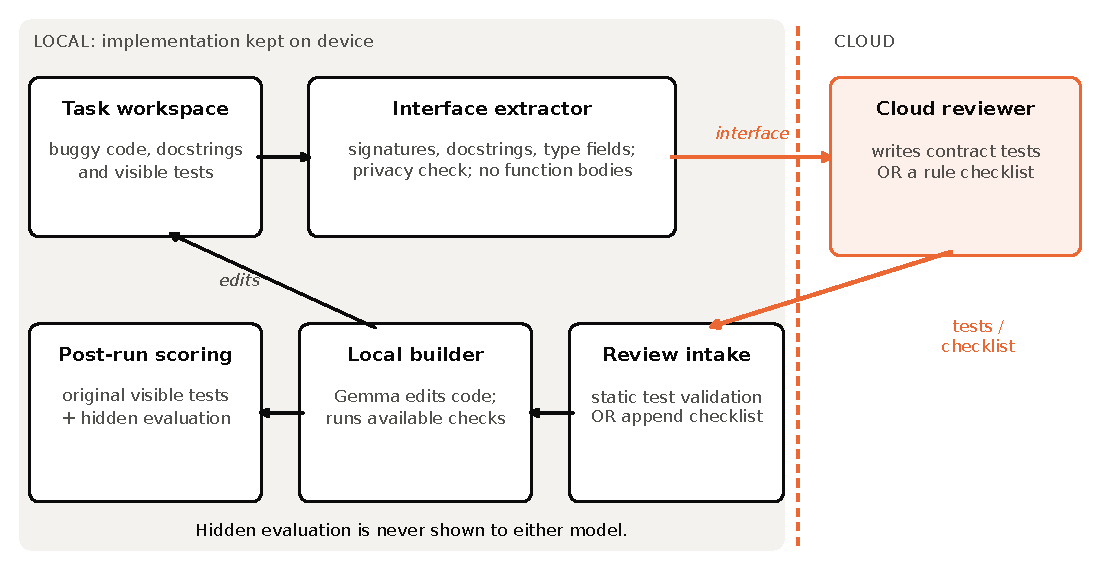
\includegraphics[width=\linewidth]{fig1_architecture.pdf}
\caption{Information flow. Only the interface (signatures, docstrings, data-type fields) crosses the boundary to the cloud, and only a statically validated unit-test module (or a rule checklist) comes back; the agent edits the code locally until its visible tests and the contract tests pass. Acceptance is decided after the run by the task's own visible tests and a hidden holdout that neither model sees.}\label{fig:architecture}
\end{figure}

% =====================================================================
\section{Experimental design}\label{sec:design}
All runs use the same agent loop, deadline and attempt limit in each arm, three seeds (303, 404, 505) per task, and alternate the order of arms per seed. Tasks are small Python repair tasks (one or two modules) in which the visible tests cover only part of the docstring; each was checked offline so that the original code and partial fixes fail and reference fixes pass both visible and hidden checks, while the original and selected partial fixes fail.

The evidence was collected in five runs on 19 tasks (\cref{tab:runs}) and two pre-registered campaigns, with 25 new specifications in A and six reused specifications in B. Runs R1--R3 were exploratory; between R3 and R4 a measurement error was found and corrected (\cref{sec:res-measurement}); R4 was pre-registered; R5 repeats R3's comparison with the corrected measurement.

\begin{table}[tb]
\centering\small
\caption{Runs on the first 19 tasks.}\label{tab:runs}
\begin{tabularx}{\linewidth}{@{}llLLL@{}}
\toprule
Run & Commit & Tasks & Arms & Purpose \\
\midrule
R1 & \code{cc938ca} & H6, H9--H13 (6) & baseline, SPEC, SPECTESTS, ASSIST & exploratory comparison \\
R2 & \code{24fbe35} & H1--H5, H7, H8 (7) & baseline, SPECTESTS v1 & harm on solved tasks \\
R3 & \code{750647e} & H1--H13 (13) & baseline, SPECTESTS v2 & same-session comparison \\
R4 & \code{7a369ac} & H14--H19 (6, fresh) & baseline, SPECTESTS v2 & pre-registered confirmation \\
R5 & \code{7a369ac}/\code{2c59e38} & H1--H13 (13) & baseline, SPECTESTS v2 & corrected-measurement repeat \\
\bottomrule
\end{tabularx}
\end{table}

\emph{Baseline} is the agent with stage hints and adaptive generation limit. \emph{SPEC} gives the agent its own task's signatures and docstrings after the visible tests pass and requires one self-check of every rule. \emph{SPECTESTS} installs cloud contract tests before the run (v1: the functions' own file only; v2: plus data-type fields and dependent modules). \emph{ASSIST} asks the cloud for step-by-step guidance after a failed attempt. Between R3 and R4 a change was made for both arms: a single stall within an attempt now leads to a fresh attempt instead of ending the subtask.

\paragraph{Pre-registration of R4.} Before any run on H14--H19 the primary endpoint (verified completion), arms, seeds, attempt limit, pairing by (task, seed) and an exact two-sided sign test were written in the project's run ledger. The ledger is a local file outside version control, so this registration is not independently time-stamped (\cref{sec:limitations}). A first attempt of R4 crashed on a hang and used the uncorrected measurement; it was discarded and rerun unchanged except for the measurement fix.

\paragraph{Statistics.} Run-level comparisons use exact two-sided sign tests on discordant (task, seed) pairs. Because runs of one task are not independent, we also analyse the per-task difference in verified rate (contract tests minus baseline, over three seeds): task-level sign test, exact sign-flip permutation test and a cluster bootstrap over tasks (20{,}000 resamples). The task-level analysis was added after an external review and is post hoc with respect to R4.

\paragraph{Confirmatory campaigns A and B.} To address the threats of \cref{sec:limitations} --- tasks and bugs written by the author after the failure mode was known, too few unseen tasks, an unrecorded cloud model and no control for the cloud's reading of the specification --- two further campaigns were registered by public commits before they were run (\cref{app:prereg}).
\begin{itemize}
\item \emph{Tasks.} Twenty-five new repair tasks (P1--P25: 8 single-module, 10 multi-file, 7 with deliberately brief, under-specified docstrings) from domains not used before (money, text, dates, units, scheduling, statistics, configuration, matrices, rate limiting, formatting). Each docstring states numbered rules, and each rule has test cases. \textbf{Which rules the visible tests cover is not chosen by the author:} a seeded coin flip per rule ($p=0.5$) decides, constrained only so that at least one visible rule fails on the buggy code. The hidden holdout checks every rule. Task content is frozen with a SHA-256 hash per task.
\item \emph{Bugs.} In Campaign A the buggy code is written by the author. In Campaign B it is written by the local model itself: for each specification, \code{gemma4:12b} implements the editable module from its docstring skeleton (generation seeds 1--5, temperature 0.8, no tests shown); the original docstrings are restored so that the defect lies only in function bodies, and the first implementation that breaks a rule becomes the task. Specifications the model implements correctly on every seed are excluded and counted.
\item \emph{Arms.} Baseline; contract tests; and a \textbf{checklist control}. The control compares review representations while holding the cloud reviewer and interface constant; it does not isolate model strength or independence. Campaign A adds an exploratory ablation of how much interface the cloud sees (signatures only; plus docstrings; full).
\item \emph{Settings.} As in R4--R5, with the cloud model pinned (Gemini 4 Argon in Campaign A; Gemini 3.8 Flash in Campaign B, by a registered amendment) and the one-time generation time recorded per task. Seeds 303, 404, 505. Primary test: exact two-sided sign test over tasks on the per-task verified rate (contract tests vs baseline); secondary: silent false successes, contract tests vs checklist, results by category, cost.
\end{itemize}

% =====================================================================
\section{Results}\label{sec:results}

\subsection{Exploratory comparison (R1)}\label{sec:res-r1}
On six specification-heavy tasks, verified completion was 7/18 for the baseline, 5/18 with local self-checks (SPEC), 16/18 with contract tests (SPECTESTS) and 8/18 with guidance after failure (ASSIST); SPECTESTS versus baseline gave 10 wins and 1 loss (run-level $p=0.012$). Runs that passed the visible tests but failed the hidden evaluation numbered 11 for the baseline, 10 for SPEC, 0 for SPECTESTS and 10 for ASSIST. R1 scored the SPECTESTS arm with a stricter criterion than the baseline (\cref{sec:res-measurement}).

\subsection{Interface completeness decides between help and harm (R2, R3)}\label{sec:res-interface}
On seven tasks the baseline already solves, the first version of the contract tests (v1), written from the functions' own file only, reduced verified completion from 21/21 to 15/21 (0 wins, 6 losses, $p=0.031$). Five losses were on H1 and H3, where the data types live in other modules; grading the generated modules against reference implementations showed 19 of 20 tests wrong for H1 (a non-existent field name) and 11 of 12 for H3 (a missing constructor argument). With data-type fields and dependent modules in the payload (v2), every generated module for the 13 tasks passed on its reference implementation, and the solved tasks lost 2 of 21 runs (not significant); on the four tasks where the baseline mostly stopped at the visible tests, verified completion rose from 2/12 to 10/12 (8 wins, 0 losses, $p=0.0078$).

\subsection{Pre-registered run on fresh tasks (R4)}\label{sec:res-r4}
On six tasks not used before, verified completion was 4/18 for the baseline and 11/18 with contract tests (8 wins, 1 loss, 9 ties; run-level $p=0.039$), and silent false successes were 14/18 and 3/18. At task level, three tasks improved (H14 0/3$\to$3/3, H15 0/3$\to$3/3, H16 0/3$\to$1/3), none worsened and three were unchanged: sign test $p=0.25$, mean gain $+0.39$ (cluster-bootstrap 95\% CI 0.06--0.72). The three remaining silent failures were all on H17; the only violated hidden rules concern empty pairs (\code{"a=1;;b=2"}, \code{"a=1;"}), a reading of the docstring that is arguably ambiguous; grading H17 without those two cases gave 7/18 versus 14/18 with the same 8 wins and 1 loss. All six generated modules passed on independent reference implementations.

\subsection{All 19 tasks with corrected measurement (R4 + R5)}\label{sec:res-19}
R5 repeated the R3 comparison on H1--H13 with the corrected measurement: 28/39 versus 37/39 (10 wins, 1 loss, run-level $p=0.012$), silent false successes 11/39 versus 0/39, and 26 of 27 SPECTESTS runs verified on the nine tasks the baseline solves 3/3 (one H6 loss). Pooled over R4 and R5 (19 tasks, identical engine and checks), verified completion was 32/57 versus 48/57 and silent false successes 25/57 versus 3/57. \Cref{tab:tasklevel} and \cref{fig:pertask} give the task-level picture; \cref{fig:silent} shows silent false successes. The gain is concentrated in seven tasks whose rules are stated only in docstrings (H9, H10, H12, H13, H14, H15, H16); eleven tasks are unchanged and one (H6) lost one of three runs.

\begin{table}[tb]
\centering\small
\caption{Task-level analysis of R4 and R5 (unit = task; difference in verified rate over three seeds, contract tests minus baseline).}\label{tab:tasklevel}
\begin{tabularx}{\linewidth}{@{}LcccL@{}}
\toprule
Set & Better/worse/equal & Sign test $p$ & Sign-flip $p$ & Mean gain (95\% cluster-bootstrap CI) \\
\midrule
\gentable{2}
\bottomrule
\end{tabularx}
\end{table}

\begin{figure}[tb]
\centering
\begin{subfigure}[t]{0.52\linewidth}\centering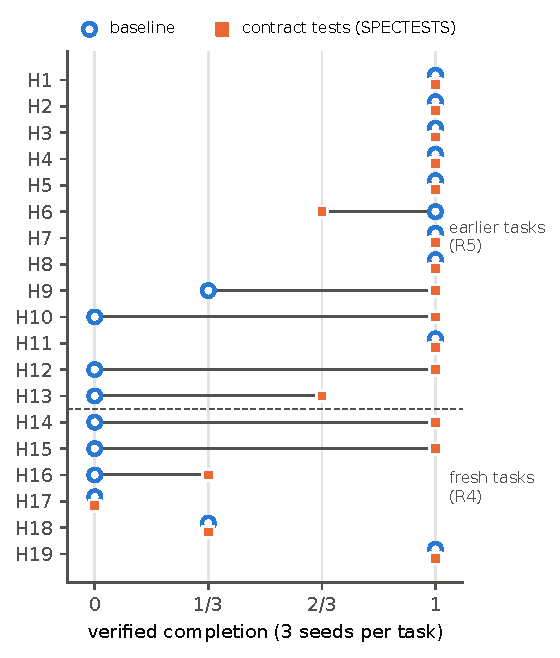
\includegraphics[width=\linewidth]{fig2_per_task.pdf}\caption{Verified completion per task.}\label{fig:pertask}\end{subfigure}\hfill
\begin{subfigure}[t]{0.46\linewidth}\centering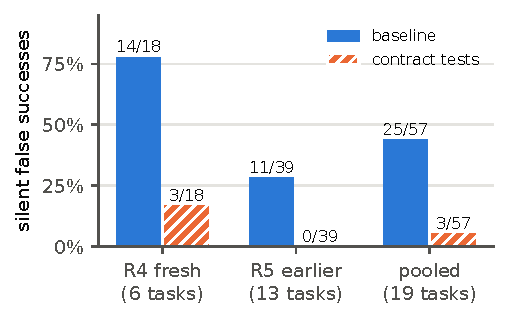
\includegraphics[width=\linewidth]{fig3_silent.pdf}\caption{Silent false successes.}\label{fig:silent}\end{subfigure}
\caption{R4 and R5. (a) Verified completion per task (three seeds) for the baseline (open circles) and with contract tests (filled squares); tasks below the dashed line are the fresh tasks of the pre-registered run R4. (b) Runs in which the agent reported success but the independent check failed.}\label{fig:r45}
\end{figure}

\subsection{Quality of the generated tests}\label{sec:res-quality}
The generated tests were examined without the agent. \textbf{Over-constraint.} Forty-seven distinct implementations that passed both the visible tests and the hidden evaluation in runs \emph{without} contract tests were reconstructed from recorded diffs (initial-state hashes checked) and run against the v2 contract modules: 6 of 91 implementation--module pairs failed, all on H4 (a negative weight must raise) and H9 (a \code{+} sign or a non-ASCII prerelease character must be rejected). In each case the docstring states the rule and the implementation violates it; the hidden evaluation does not test it. We found no contract test that requires behaviour the docstring does not state. \textbf{Mutation coverage.} Of 448 single-point AST mutants of reference implementations (19 tasks), the hidden evaluation killed 333; of those, the visible tests killed 205 (61.6\%) and the v2 contract modules killed all (469 of 469 evaluated mutant--module pairs; a mutant can be paired with more than one generated module, so this denominator differs from 333 unique mutants; \cref{fig:mutation}). A further 84 mutants survived the hidden evaluation but were killed by contract tests; each violates a docstring rule on inspection. Thirty-one mutants survived every check. For H14--H16 the reference was a holdout-passing implementation from a contract-test run, because no baseline run solved those tasks. A consequence is that the hidden evaluations are weaker than the specifications, so ``verified'' overstates correctness in both arms; since the contract tests enforce the missed rules, this bias favours the baseline.

\begin{figure}[tb]
\centering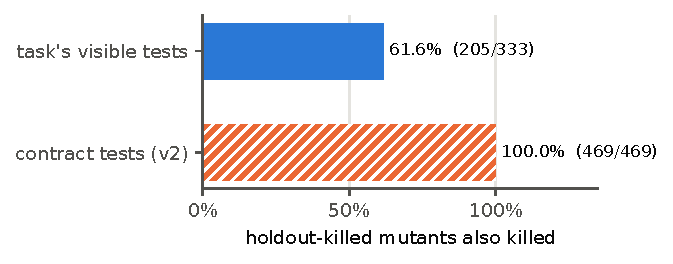
\includegraphics[width=0.78\linewidth]{fig4_mutation.pdf}
\caption{Of the single-point mutants that the hidden evaluation kills, the share also killed by the task's visible tests and by the v2 contract tests (contract counts are mutant--module pairs).}\label{fig:mutation}
\end{figure}

\subsection{Measurement correction and cost}\label{sec:res-measurement}
In R1--R3 the independent visible check for the SPECTESTS arm also ran the generated tests, and the hidden evaluation ran only if that check passed; SPECTESTS runs were therefore scored against a stricter criterion than baseline runs, which can only have lowered their scores. R4, R5 and both campaigns use the corrected checks (the task's own tests only, hidden evaluation always run, hangs counted as failures).

Contract tests make runs longer: in R4 the summed wall time was 929\,s versus 4{,}014\,s and local tokens 256{,}017 versus 1{,}171{,}194, plus 91{,}958 cloud tokens for six generation calls; in R5, 3{,}092\,s versus 5{,}273\,s and 614{,}904 versus 1{,}378{,}211 local tokens, plus about 264{,}000 cloud tokens for 13 tasks. The baseline is fast partly because it stops as soon as the weak visible tests pass. These wall-time figures exclude the one-time cloud generation per task, which was not timed in R1--R5; the ratios (1.7--4.3$\times$) are lower bounds on end-to-end cost. The campaigns record generation time separately.

\subsection{Interventions that did not help}\label{sec:res-negative}
\begin{itemize}
\item \textbf{Self-checking by the same model} (SPEC, R1): 5/18 versus 7/18; the agent's self-checks exercised only behaviour it had already implemented.
\item \textbf{Cloud guidance after failure} (ASSIST, R1): 8/18; guidance is triggered by a failed attempt, and the first attempt usually passed the visible tests, so it triggered once in 18 runs.
\item \textbf{Escalation of generation limit, thinking on retry and cloud assistance} in a two-attempt ladder: on H6--H8 the differences came from one task and were attributed to run-to-run variation.
\item \textbf{One-step harness adaptation} in the style of Harness$^2$~\citep{harness2}: on held-out tasks the default harness verified 7/12 runs and the adapted harnesses 6/12, with longer total wall time (829\,s versus 601\,s); the standard and verifier-gated promotion rules made the same choices on every task, so the experiment does not distinguish them.
\end{itemize}

\subsection{Campaign A: 25 new tasks with seeded rule visibility (pre-registered)}\label{sec:res-a}
All 225 primary runs were completed (3 arms $\times$ 25 tasks $\times$ 3 seeds). Each of the 25 test modules and 25 checklists was generated once with Gemini 4 Argon and reused across seeds (\cref{tab:campaign-a}, \cref{fig:campaign-a}).

\begin{table}[tb]
\centering\small
\caption{Campaign A, all runs (25 tasks $\times$ 3 seeds). Generation is the one-time cloud call per task.}\label{tab:campaign-a}
\begin{tabularx}{\linewidth}{@{}Lrrrrr@{}}
\toprule
Arm & Verified & Silent false successes & Run wall time & Generation & Cloud tokens \\
\midrule
\gentable{3}
\bottomrule
\end{tabularx}
\end{table}

\begin{figure}[tb]
\centering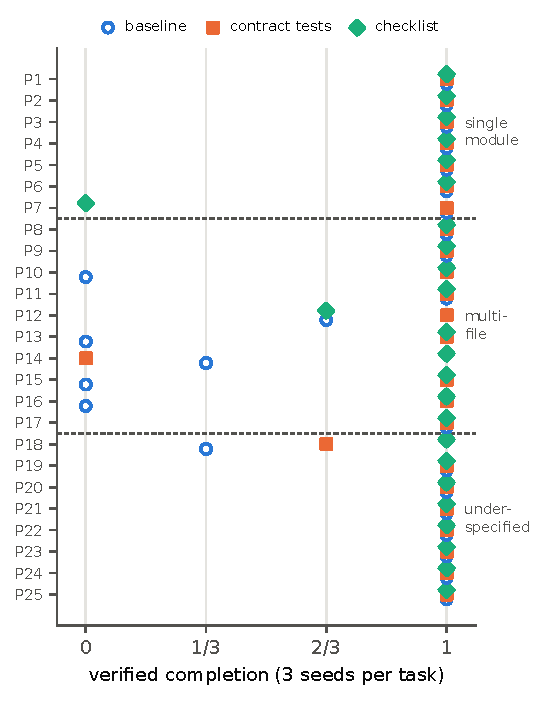
\includegraphics[width=0.55\linewidth]{fig5_campaign_a.pdf}
\caption{Campaign A: verified completion per task (three seeds) for the baseline (open circles), contract tests (squares) and the checklist control (diamonds). Dashed lines separate single-module, multi-file and under-specified tasks.}\label{fig:campaign-a}
\end{figure}

\paragraph{Primary hypothesis (H1) not confirmed.} At task level, contract tests improved 6 tasks and worsened 1 (18 unchanged): sign test $p=0.125$, sign-flip permutation $p=0.0625$, mean gain in verified rate $+0.17$ (cluster-bootstrap 95\% CI 0.04--0.33). The direction matches the earlier runs, but the registered test does not reach $\alpha=0.05$. Silent false successes (H2) were lower on 3 tasks and higher on none ($p=0.25$).

The positive bootstrap interval for the mean and the non-significant sign test are not contradictory. The sign test uses only the direction of non-zero task effects, whereas the bootstrap targets their mean magnitude using the empirical task sample. The registered sign test remains the primary decision rule; the interval is not a substitute for it.

\paragraph{No detected advantage over the checklist (H3).} The checklist matched the aggregate verified-completion rate of executable contract tests (71/75) and silent false successes (1/75). Outcomes differed by task: tests versus checklist gave 2 better, 2 worse and 21 equal ($p=1.0$). No equivalence or non-inferiority margin was registered or tested; a non-significant difference does not establish either. The comparison shows that an executable review was not necessary to obtain these aggregate outcomes, without isolating why either review helped.

\paragraph{Where the effect sits.} For contract tests versus baseline, all changes were in the 10 multi-file tasks (6 better, 1 worse; mean $+0.43$). The baseline already passed every run on the 8 single-module and 7 under-specified tasks. This ceiling leaves only seven discordant tasks for the primary sign test. The checklist separately harmed the single-module CSV task P7 (below). No task without hidden failing rules was harmed by contract tests.

\paragraph{Failures of the two cloud arms.} P14 with contract tests failed 3/3 by running out of attempts while the (correct) contract tests still failed; P7 with the checklist failed 3/3 the same way after the checklist spelled out the quoting rules of CSV; both are explicit failures. For P18 both generated test modules were rejected by the static validator (they used \code{\_\_dict\_\_}), so the contract-test arm ran without tests on that task, as registered.

\paragraph{Generation reliability.} A valid module was installed on 24/25 tasks (96\%); one task (P18, 4\%) had no installed module after both allowed generation attempts were rejected. This is a task-level rejection rate, not a per-reply rate. The three P18 runs remain in the intention-to-treat analysis. A cloud backend failure stops the runner; static rejection is a method outcome.

\paragraph{Quality of the generated tests.} Run against the reference fixes, 4 tests in 3 of the 24 installed modules failed: three are over-constrained --- on the under-specified P20 they require \code{ValueError} for an empty list and a float result, and on P12 a test requires the delegation to \code{statcore.mean} to be visible to monkey-patching, which depends on the import style rather than behaviour; the fourth (P10) expects a float \code{0.0} where the docstring says 0.0 and the reference returns the integer 0. None of these tests caused a failed run.

\paragraph{How much interface the cloud needs (exploratory ablation, seed 303).} With signatures alone, contract tests left verified completion at the baseline level (19/25, 2 silent; baseline 20/25 on this seed); adding docstrings gave 25/25 (0 silent); the full interface with type fields gave 23/25 (1 silent). On these tasks the value lies in the docstrings; type fields added nothing here, whereas on H1 and H3, whose data types live in separate modules, their absence produced impossible tests (\cref{sec:res-interface}). One seed per level, so differences of one or two runs are within run-to-run variation.

\paragraph{Cost including generation.} Summed run time plus one generation per task was 6{,}674.85\,s for baseline, 10{,}255.96\,s for contract tests and 7{,}459.95\,s for the checklist: campaign overheads of 53.7\% and 11.8\%, respectively. Run time alone increased by 44.3\% and 4.6\%. Each generated artifact was reused for three seeds, so these are amortised campaign costs, not measured overheads for a one-off deployment. They exclude software setup, analysis and human effort, and do not measure energy or monetary cost. Generation was not timed in R1--R5; their run-time ratios cannot be compared as complete end-to-end costs.

\subsection{Campaign B: bugs written by the local model (pre-registered; descriptive)}\label{sec:res-b}
\paragraph{Construction.} Asked to implement each of the 25 Campaign A specifications from its docstring skeleton, \code{gemma4:12b} produced a correct module on all five generation seeds for 19 specifications (104 generations; one rejected as incomplete). Only six specifications yielded a natural bug (N1, N7, N8, N9, N13, N18), fewer than the registered threshold of ten, so Campaign B is reported descriptively, as registered. In four of the six the coin flip made every broken rule visible; only N7 and N18 have rules broken in hidden-only form. With numbered rules in the docstring, the local model rarely leaves a stated rule unimplemented when it writes the code from scratch; the silent failures of the earlier tasks arose when it repaired code against incomplete tests.

\paragraph{Results.} All 54 runs were completed with Gemini 3.8 Flash as the cloud model (\cref{tab:campaign-b}). On N18 contract tests were verified in 3 of 3 runs, the checklist in 1 of 3 and the baseline in none; on N13 only the checklist helped (2 of 3); N7, whose generated parser loops on some inputs, was not solved by any arm. All six generated test modules passed on the reference fixes. With six tasks these results are descriptive; they point the same way as Campaign A, with the contract tests the only arm without a silent false success.

\begin{table}[tb]
\centering\small
\caption{Campaign B, all runs (6 tasks $\times$ 3 seeds; descriptive).}\label{tab:campaign-b}
\begin{tabularx}{\linewidth}{@{}Lrrrrr@{}}
\toprule
Arm & Verified & Silent false successes & Run wall time & Generation & Cloud tokens \\
\midrule
\gentable{5}
\bottomrule
\end{tabularx}
\end{table}

\subsection{Pooled evidence (post hoc)}\label{sec:res-pooled}
Pooling every run made with the corrected measurement --- R4, R5 and Campaigns A and B, 50 tasks, contract tests against the baseline on the same task and seed --- gives the overall size of the effect (\cref{tab:pooled}). This analysis was decided after the runs and is reported as descriptive support, not as a registered test. At run level within Campaign A, contract tests fixed 15 runs the baseline failed and broke 2 ($p=0.002$), and the checklist fixed 17 and broke 4 ($p=0.007$); both removed 9 of the 10 discordant silent false successes ($p=0.02$). Runs with different seeds of one task are not independent, so the run-level values overstate the evidence for new tasks; the task-level values address within-task seed dependence; shared specifications require the additional sensitivity below.

\paragraph{Shared-specification sensitivity (post hoc).} The 50 instances comprise 19 earlier tasks, 25 Campaign A tasks and 6 Campaign B variants of A specifications. Grouping each Pk with its Nk variant gives 44 originating-specification groups. We pool runs within each group and give groups equal weight in a sign test: verified completion improves in 13 groups and worsens in 2 ($p=0.00739$); silent false successes decrease in 12 groups and increase in none ($p=0.000488$). This sensitivity does not establish independence between all groups. It addresses one known dependency and leaves the pooled analysis exploratory. Script: \code{scripts/analysis/publication.py}.

\begin{table}[tb]
\centering\small
\caption{Pooled runs with corrected measurement (50 tasks $\times$ 3 seeds; post hoc).}\label{tab:pooled}
\begin{tabularx}{\linewidth}{@{}Lrrr@{}}
\toprule
Outcome & Baseline & Contract tests & Tasks improved/worsened (sign test $p$) \\
\midrule
\gentable{4}
\bottomrule
\end{tabularx}
\end{table}

% =====================================================================
\section{Discussion}\label{sec:discussion}
\paragraph{A coverage gap in the stopping criterion.} The observed failures are consistent with insufficient coverage of the stopping criterion: the agent often stopped after visible tests passed while leaving docstring rules unimplemented. Alternative interventions did not demonstrate reliable gains under the specific tasks and budgets tested (\cref{sec:res-negative}); this is not evidence that these interventions are ineffective in other settings.

\paragraph{What the control establishes.} The checklist and executable tests produced the same Campaign A aggregate outcomes, with lower measured campaign time for the checklist (11.8\% versus 53.7\% overhead including generation). This is consistent with a benefit from explicitly presenting specification requirements. The study does not separately identify the contributions of reviewer independence, model capability, structured presentation, extra explicit information or timing. In particular, SPEC was a local self-check after visible success, not a local checklist generated before repair. Its failure does not show that independence and model strength are each necessary. A future registered comparison should hold timing and interface constant and compare a pre-repair local checklist, a cloud checklist and a direct presentation of the original rules. Tests remain executable audit artifacts, but no additional completion benefit over the checklist was detected here; equivalence was not established.

\paragraph{Disclosure and over-constraint.} The one-seed ablation suggests that docstrings carried useful information beyond signatures. Type fields were necessary for some earlier tasks but added no measured gain in Campaign A. Incomplete, ambiguous or implementation-sensitive requirements can lead to over-constrained tests, including P12 outside the under-specified category. No observed failed run was attributed to the adjudicated over-constraints; that does not establish their harmlessness in other settings.

\paragraph{Scope and next validation.} Contract-test gains in Campaign A were concentrated in multi-file tasks; many simpler tasks had a ceiling baseline. This motivates a future selective-review policy, but neither an automatic selector nor a deployment cost bound was evaluated. A stronger external validation would freeze a new set of real repository defects with independent reference fixes and tests, and report results separately from the designed tasks here.

\paragraph{Strength of the evidence.} The effect points the same way in every experiment, and pooled over all corrected runs it is large: silent false successes fell on 12 tasks and rose on none, and failures fell on 14 tasks and rose on 2 (\cref{tab:pooled}). The registered task-level test of Campaign A alone did not reach significance (6 better, 1 worse, $p=0.125$), because the baseline already solved 15 of the 25 tasks and only seven were discordant. We therefore present the size and consistency of the effect as the main result and the registered test as a limit on how far it has been confirmed on new tasks.

% =====================================================================
\section{Limitations and threats to validity}\label{sec:limitations}
\begin{itemize}
\item \textbf{Task selection.} All tasks are small Python repair tasks written by the author. The 19 earlier tasks were partly written \emph{after} the failure mode had been identified and over-represent tasks where the method helps. Campaign A reduces this bias (which rules are visible is decided by a seeded coin flip) and Campaign B takes the bugs from the local model, but the specifications themselves are still the author's, with rules stated explicitly and numbered, which makes them easier than typical real-world docstrings. The effect size on naturally occurring bugs is unknown.
\item \textbf{Development reuse.} Tasks H1--H13 were used while developing the mechanism; R4 and Campaign A use new tasks; Campaign B has newly generated buggy implementations of six Campaign A specifications, not new specifications.
\item \textbf{Statistical unit and power.} Seeds of one task are not independent; run-level $p$-values overstate generalisation to new tasks. Task-level tests for R4--R5 (\cref{tab:tasklevel}) are post hoc; in Campaign A the registered task-level test was not significant, largely because the baseline already solved most tasks.

\item \textbf{Causal identification and shared specifications.} Review generation changes model, representation, information and timing together. The local SPEC comparison is not a matched pre-repair checklist control. Six Campaign B tasks reuse A specifications, so 50 task instances are not 50 independent specifications; the 44-group sensitivity is post hoc.
\item \textbf{Pre-registration.} R4's registration lives in a local ledger outside version control and is not independently time-stamped; Campaigns A and B were registered by public commits before they ran, with one documented amendment to Campaign B (cloud model).
\item \textbf{Ground truth.} Hidden evaluations are weaker than the docstrings (\cref{sec:res-quality}); verified rates are upper bounds for both arms.
\item \textbf{Scope: one model stack.} This is a study of one stack --- Gemma as the local builder, a cloud model behind the Antigravity CLI as the reviewer. Google's announcement pairs Gemma 4 26B A4B with Gemini 3.8 Flash~\citep{kotwani2026antigravity}; we use the smaller \code{gemma4:12b}, Gemini 4 Argon in Campaign A and Gemini 3.8 Flash in Campaign B. In R1--R5 the CLI's default model was used and not recorded, so those runs are not claimed to use Gemini. No claim is made for other model families, and comparisons between Campaigns A and B are descriptive.
\item \textbf{Hardware.} One consumer GPU with partial CPU offload; wall time is sensitive to background load.
\item \textbf{Cost accounting.} Cloud generation time is missing from R1--R5.
\item \textbf{Interrupted runs.} R5 and Campaigns A and B were paused at the author's request and resumed from saved results with the same generated tests and checklists, in different sessions.
\end{itemize}

% =====================================================================
\section{Data and code availability}\label{sec:availability}
Code and artifacts are available at \url{https://github.com/cyberdid/cloud-edge-ai-orchestrator} on \code{main}. The frozen experimental-data snapshot is commit \code{9cd894f717a4235c7cb7bdc36563275ba36bdb0f}; the revised publication package is identified by tag \code{paper-i-preprint-2026-10-21-rev2}. File checksums and exact reproduction instructions are in \code{docs/paper/README.md}. From the repository root, \code{bash scripts/paper/reproduce.sh} recomputes summaries, figures and both language PDFs from saved results without model calls. Numerical table bodies are generated by \code{docs/paper/tex/gen\_tables.py}; \cref{app:evidence} maps results to files. No archival DOI is claimed in this version.

% =====================================================================
\section{Conclusion}\label{sec:conclusion}
A local 12B coding agent can report success after passing incomplete visible tests. In this bounded repair-task study, adding cloud-generated contract tests from an interface-only specification reduced silent false successes from 37/150 to 4/150 and raised measured verified completion from 66.0\% to 87.3\% (pooled, post hoc). A checklist matched the aggregate verified-completion rate of tests in Campaign A, with 11.8\% versus 53.7\% additional campaign time including generation; equivalence was not established. The registered task-level test did not reach significance. Results motivate further specification-review research, while leaving causal attribution and generalisation to independent real-world defects open.

\section*{Research transparency}
\textbf{License.} Article text, figures and experimental records: Creative Commons Attribution 4.0 International (\url{https://creativecommons.org/licenses/by/4.0/}); executable source: Apache License 2.0. The repository licensing guide defines scope and third-party exceptions.
\textbf{Author status and collaboration.} The author is an independent researcher and PhD student at the State University of Trade and Economics; the stated cooperation with the Department of Software Engineering and Cybersecurity is confirmed by the author. The experiments ran on the author's equipment and accounts. Cooperation does not imply Google participation or endorsement.

\textbf{Use of AI tools.} AI assistants supported software development, analysis implementation, drafting, translation and typesetting. The evaluated models and experiment settings are reported separately. AI-generated feedback and static or numerical checks are not independent human peer review or an independent experimental replication. The author is responsible for the final claims, references and publication decision.

\bibliographystyle{plainnat}
\bibliography{../refs}

% =====================================================================
\appendix

\section{Pre-registrations and deviations}\label{app:prereg}
\begin{itemize}
\item \textbf{Campaign A} was registered in \code{docs/paper/PREREGISTRATION\_CAMPAIGN\_A.md} (commit \code{5c9ac2f}, pushed 2026-10-20 12:52 +03:00) before any run; the task set P1--P25 was frozen in \code{scripts/paper\_tasks/manifest.json} (commit \code{24ea7a0}). Deviations: the campaign was paused twice at the author's request and resumed from saved results; the analysis script was later changed to skip categories without tasks (needed for Campaign B), which does not change any Campaign A output.
\item \textbf{Campaign B} was registered in \code{docs/paper/PREREGISTRATION\_CAMPAIGN\_B.md} (commit \code{214f0a8}) before generation; Amendment~1 (commit \code{60dacd5}, before generation) changed the cloud model to Gemini 3.8 Flash because of the Gemini 4 Argon quota and added a stop on failed cloud calls. The generated tasks were frozen in \code{scripts/paper\_tasks/natural\_tasks.json} (commit \code{d2f2807}) before any repair run. Six tasks remained, below the registered threshold of ten, so the campaign is reported descriptively, as registered.
\item \textbf{R4} was registered in a local ledger (not time-stamped); a first attempt that crashed on a hang was discarded and rerun with the measurement fix.
\end{itemize}

\clearpage
\section{Evidence map}\label{app:evidence}
\begin{table}[!ht]
\centering\small
\begin{tabularx}{\linewidth}{@{}P{0.27\linewidth}L@{}}
\toprule
Result & Files in the repository \\
\midrule
R1 (\cref{sec:res-r1}) & \code{benchmarks/spec\_contract\_experiment.json}; \code{docs/SPEC\_CONTRACT\_RESULTS.md} \\
R2, R3 (\cref{sec:res-interface}) & \code{benchmarks/spec\_contract\_control.json}, \code{benchmarks/spec\_contract\_v2.json} \\
R4 (\cref{sec:res-r4}) & \code{benchmarks/spec\_contract\_confirm\_fresh.json} \\
R5 (\cref{sec:res-19}), \cref{tab:tasklevel} & \code{benchmarks/spec\_contract\_confirm\_all.json}; \code{scripts/analysis/clustered\_spec.py} \\
Test quality (\cref{sec:res-quality}) & \code{benchmarks/oracle\_quality.json}; \code{scripts/analysis/oracle\_quality.py} \\
Negative results (\cref{sec:res-negative}) & \code{benchmarks/gemma\_orion\_phase2b\_escalation\_ladder.json}, \code{benchmarks/harness2\_experiment.json} \\
Campaign A (\cref{sec:res-a}) & \code{benchmarks/campaign\_a.json}, \code{campaign\_a\_ablation.json}, \code{campaign\_a\_analysis.txt}, \code{campaign\_a\_test\_grading.json} \\
Campaign B (\cref{sec:res-b}) & \code{scripts/paper\_tasks/natural\_tasks.json}; \code{benchmarks/campaign\_b.json}, \code{campaign\_b\_analysis.txt}, \code{campaign\_b\_test\_grading.json} \\
Revision checks & \code{benchmarks/publication\_analysis.json}; \code{scripts/analysis/publication.py} \\
Pooled (\cref{sec:res-pooled}) & \code{benchmarks/pooled\_analysis.txt}; \code{scripts/analysis/pooled.py} \\
System (\cref{sec:system}) & \code{antigravity\_hybrid\_orchestrator/engine/spec\_tests.py}, \code{privacy/assist\_payload.py}; \code{scripts/benchmark\_gemma\_orion\_phase2b.py} \\
Tasks P1--P25 & \code{scripts/paper\_tasks/}; \code{tests/test\_paper\_tasks.py} \\
Figures & \code{scripts/analysis/paper\_figures.py}, \code{paper\_diagram.py} \\
\bottomrule
\end{tabularx}
\end{table}

\end{document}
